\pagenumbering{Roman}    % a, b, c, ...
\thispagestyle{empty}
% نحوه درج کردن لوگوی دانشگاه
\begin{figure*}[!h]
\centerline{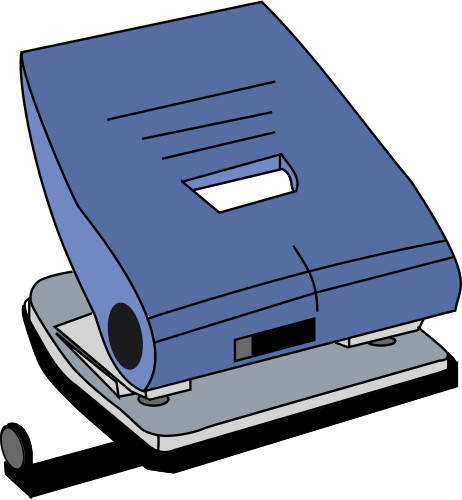
\includegraphics[width=4cm]{logo}}
%\caption{}
\end{figure*}
\begin{center}
%دستوری برای کم کردن فاصله بین لوگو و خط پایین آن
\vspace{-.8cm}

% {\large پژوهشگاه بین المللی زلزله شناسی و مهندسی زلزله}
%دستوری برای تعیین فاصله بین دو خط


\\[1cm]
بنام خدا
\\[1cm]
راهنمای کاربری
\\[.8cm]
% {\nastaliq
\begin{Huge}
نرم افزار 
\lr{CivilTools}
\end{Huge}

\\[.5cm]
\begin{latin}
    \textbf{Ver. 5.0}
\end{latin}



\begin{figure}[ht]
    \centering
        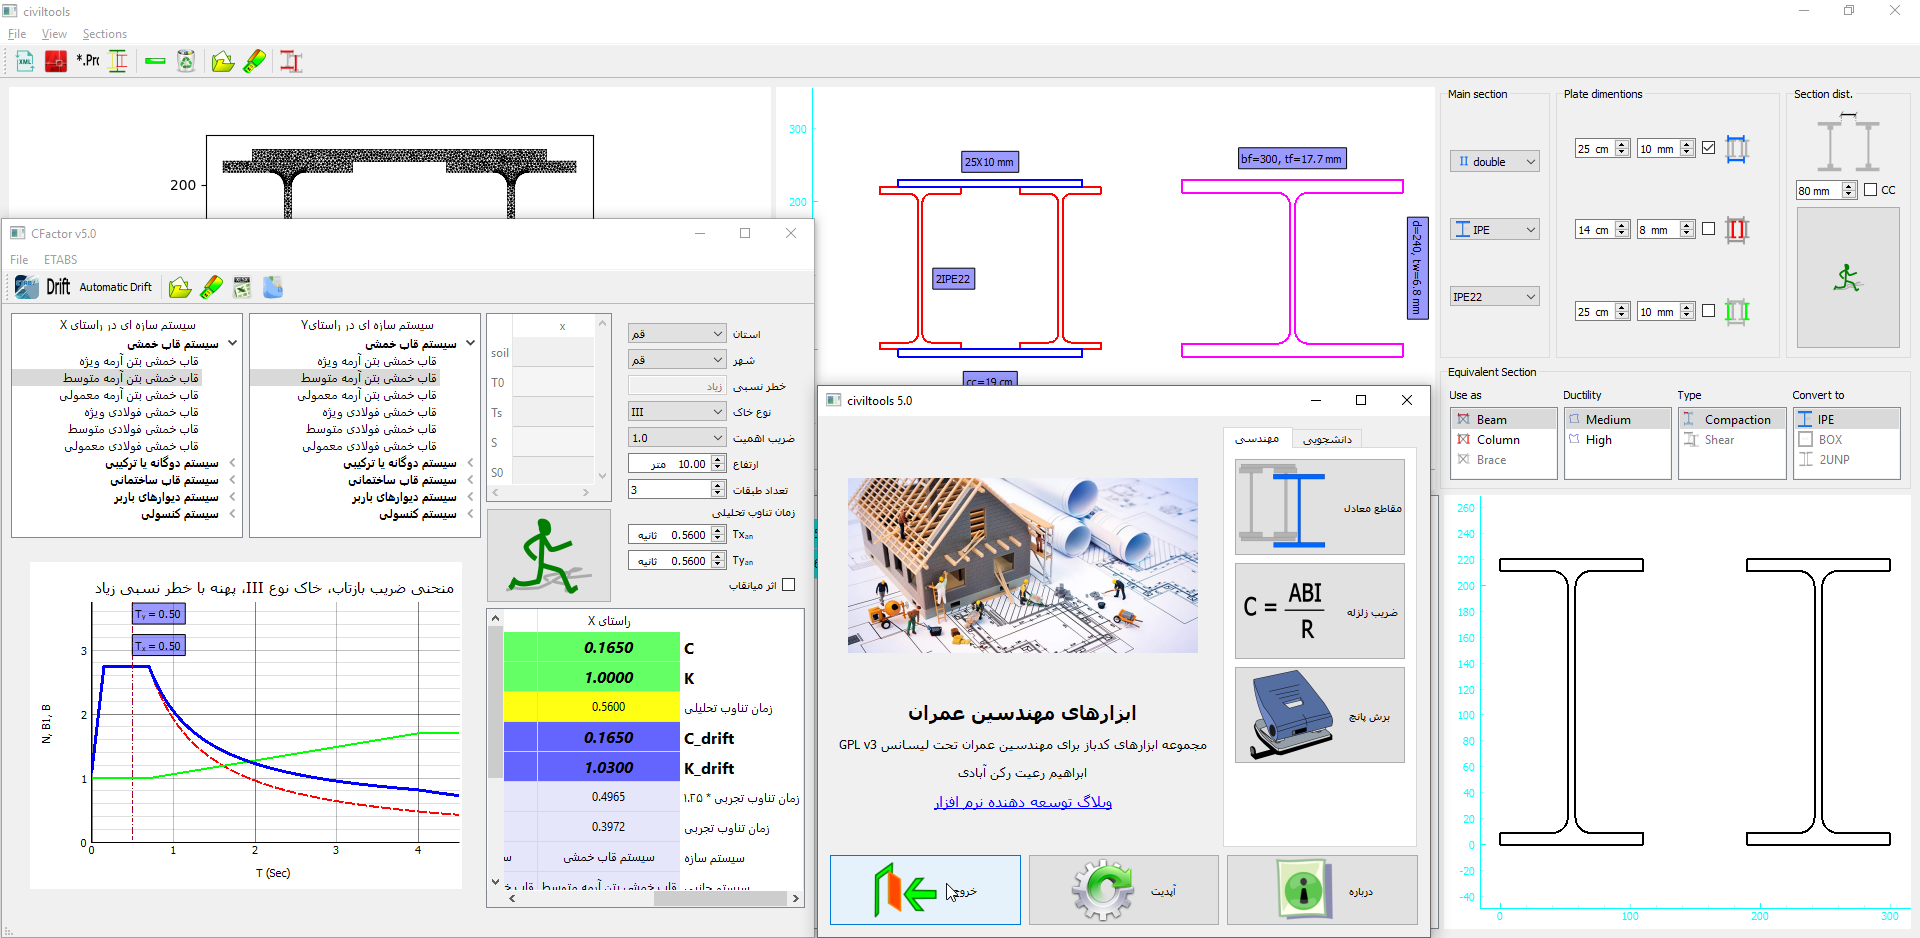
\includegraphics[width=\linewidth]{figures/civiltools}
        % \caption{DL, units:[m,kN]}
        % \label{dl-unitsmkn}
\end{figure}

\\[2.5cm]{ توسعه دهنده:}
\\[.3cm]
\textbf{{\large  \developer}}

% \\[2cm]{کارفرما}
% \\[.3cm]
% \textbf{{\large \karfarma}}
% \\ \textit{\address}

\\[1.cm]
\today
\end{center}
%\maketitle
%دستوری برای رفتن به صفحه جدید
\newpage
\thispagestyle{empty}
% \pagenumbering{Roman}   % i, ii, iii, iv, ...
\setcounter{page}{1}
\tableofcontents
% \listoffigures
% \listoftables
\newpage
